\section{Algorithmic Contribution}
\label{sec:background}

\begin{figure*}[t!]
    \centering
    \subfloat[]{
            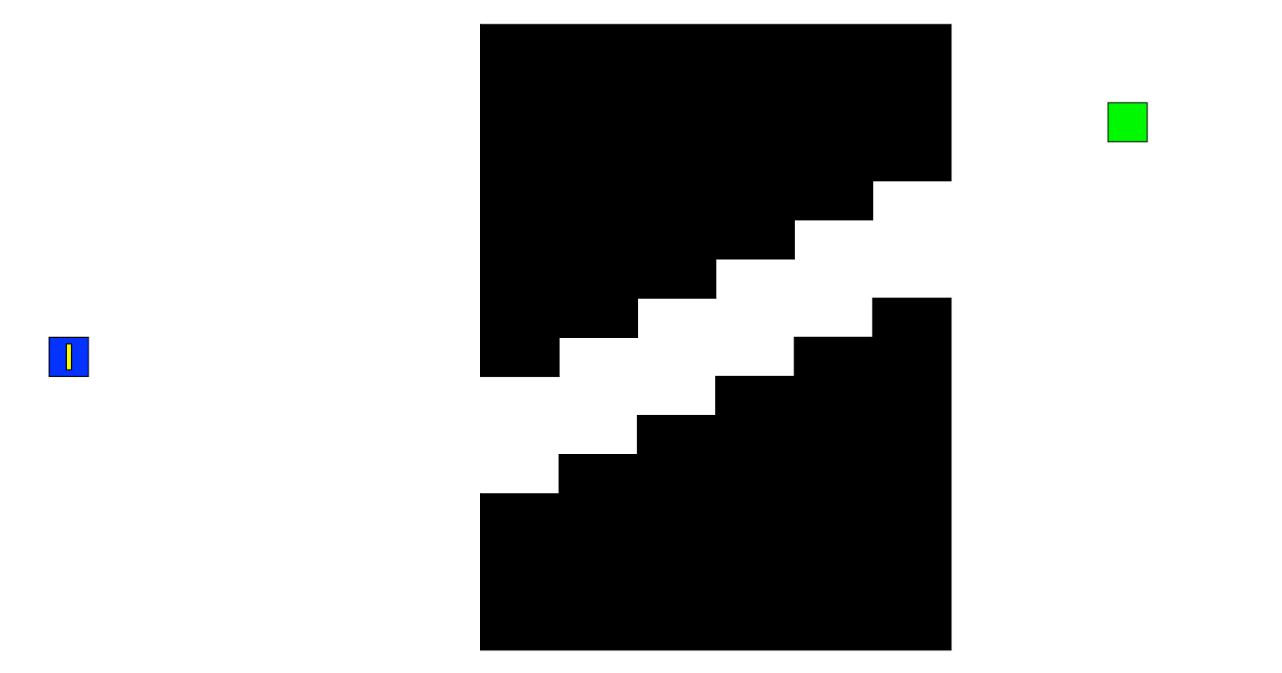
\includegraphics[width=0.39\textwidth]{figs/diag_map}
            \label{fig:diag_map}
        }
        \subfloat[]{
            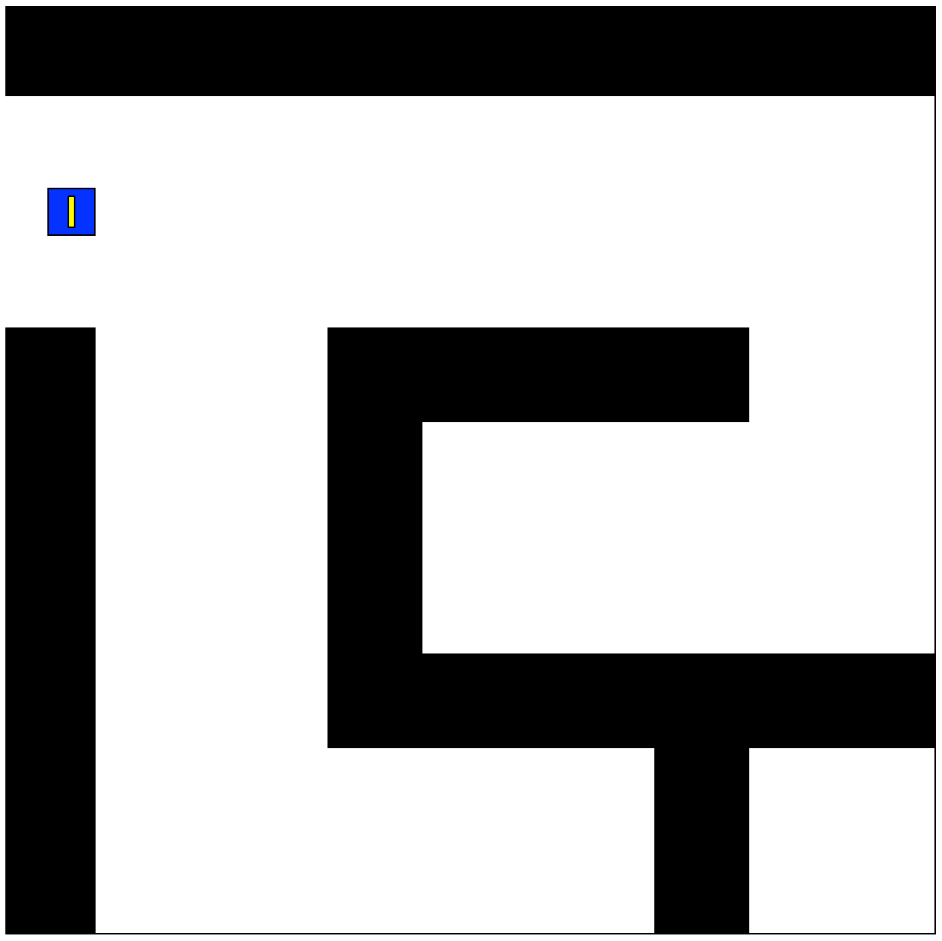
\includegraphics[width=0.2\textwidth]{figs/partial_map} 
            \label{fig:partial_map}
        }
        \subfloat[] {
            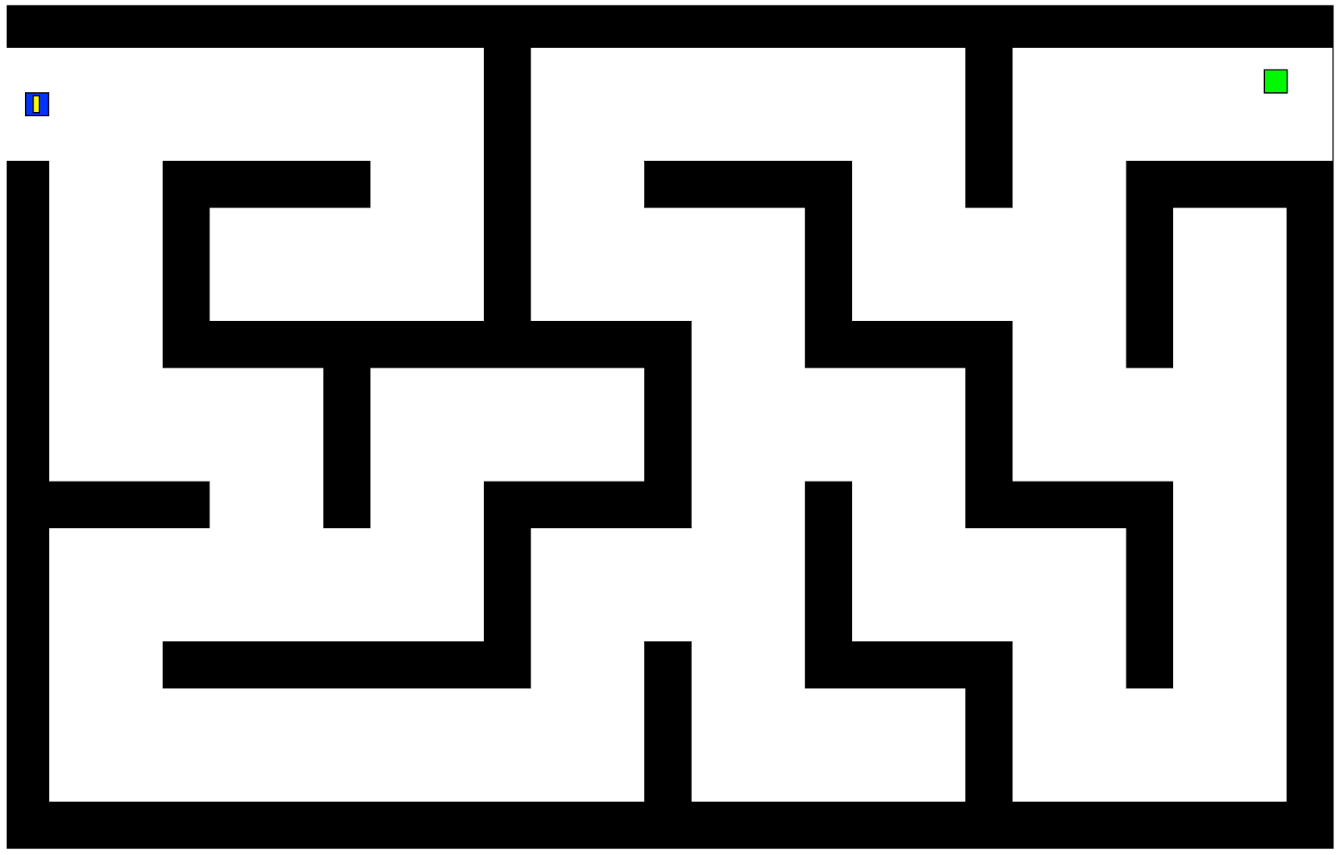
\includegraphics[width=0.315\textwidth]{figs/full_map}
            \label{fig:full_map}
        }
         \caption{\protect\subref{fig:diag_map}~Practice map for user study. \protect\subref{fig:partial_map}~Partially visible map where the field of view changes as the robot moves. \protect\subref{fig:full_map}~Fully visible map where the position of the robot and goal are always visible.}
         \label{fig:maps}
\end{figure*}

Herlant et. al determined the optimal mode by running Dijkstra's algorithm on a 2D workspace $\mathcal{W} \subset \mathbb{R}^2$ augmented by mode $m \in \mathcal{M}, \mathcal{M} = \{m_h, m_v\}$. $m_h$ is the mode that allows the robot to move horizontally and $m_v$ is the mode that allowed the robot to move vertically. Everytime the user moved the robot to a new position $(x_{new},y_{new})$ they determined the optimal mode by running Dijkstra's algorithm to find the cost $c((x_{new}, y_{new}, m),(x_g, y_g))~\forall m \in \mathcal{M}$. Note, that the mode at the goal position is irrelevant. The optimal mode $m\text{*} = \argmin_{m} c((x_{new}, y_{new}, m),(x_g, y_g))$.

Continuously running Dijkstra's algorithm is inefficient as one state can be re-expanded multiple times. Our variation of the time-optimal mode switching algorithm, utilizes Dijkstra's algorithm but only runs it once as a pre-processing phase. $c((x_{new}, y_{new}, m),(x_g, y_g))$ gives the cost of the shortest path from $(x_{new}, y_{new}, m)$ to $(x_g, y_g)$. However, if we run Dijkstra's algorithm once backward from $(x_g, y_g)$ till every state has been explored, we can get a cost from every $(x, y, m),~\forall m\in \mathcal{M}$ to the goal. This method allows use to generate an \textit{optimality map} that we can simple query at every timestep to get the optimal mode. 

This approach does not have a significant impact on the efficiency of the simulation. However, if this algorithm was extended to a higher-dimensional robot, such as the Kinova JACO, there would be a significant improvement in the time taken to find the optimal mode. 